\documentclass[tikz, border=12pt]{standalone}
\usepackage[utf8]{inputenc}
\usepackage[T5]{fontenc}
\usepackage{lmodern}
\usepackage{xcolor}
\usepackage{graphicx}
\usetikzlibrary{positioning, calc, arrows}

\definecolor{boxBorder}{RGB}{180, 195, 215}
\definecolor{t1Bg}{RGB}{242, 250, 245}
\definecolor{t2Bg}{RGB}{242, 247, 255}
\definecolor{t3Bg}{RGB}{254, 248, 240}
\definecolor{t4Bg}{RGB}{248, 245, 255}

\definecolor{greenTitle}{RGB}{27, 94, 32}
\definecolor{blueTitle}{RGB}{30, 58, 138}
\definecolor{amberTitle}{RGB}{160, 75, 5}
\definecolor{purpleTitle}{RGB}{95, 30, 180}
\definecolor{arrowColor}{RGB}{50, 65, 85}

\begin{document}
\begin{tikzpicture}[
  >=stealth,
  font=\sffamily,
  tierCard/.style={
    draw=boxBorder,
    line width=1.0pt,
    rounded corners=8pt,
    align=center,
    inner sep=8pt,
    minimum width=16.0cm
  },
  flowArrow/.style={
    ->,
    line width=1.5pt,
    draw=arrowColor
  },
  biArrow/.style={
    <->,
    line width=1.5pt,
    draw=arrowColor
  },
  tagLbl/.style={
    font=\small\bfseries,
    fill=white,
    inner sep=3.5pt,
    rounded corners=3pt,
    draw=gray!35,
    line width=0.5pt,
    text=arrowColor
  }
]

% ==================== TẦNG 1: TẦNG ĐEO ====================
\node[tierCard, fill=t1Bg] (t1) at (0, 0) {
  {\bfseries\large\color{greenTitle} TẦNG 1: TẦNG ĐEO (WEARABLE TIER)}\\[6pt]
  \begin{tikzpicture}
    \node[draw=gray!30, fill=white, rounded corners=5pt, inner sep=4pt] (p1) at (-4.5, 0) {
      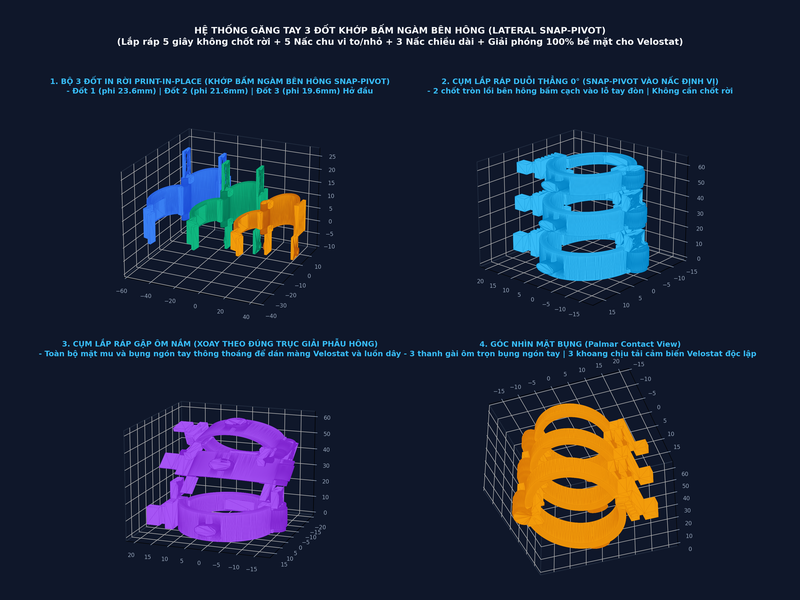
\includegraphics[width=4.5cm, height=2.5cm, keepaspectratio]{assets/splint_3d.png}
    };
    \node[draw=gray!30, fill=white, rounded corners=5pt, inner sep=4pt] (p2) at (4.5, 0) {
      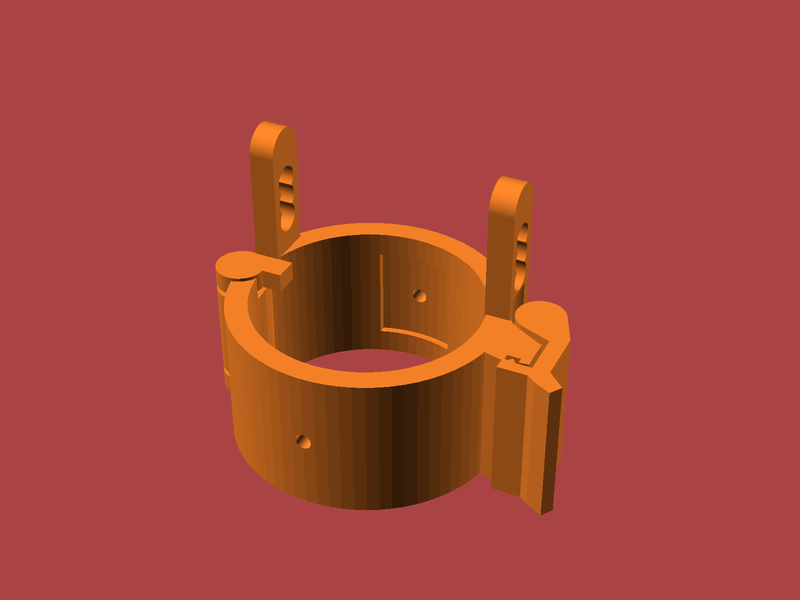
\includegraphics[width=4.5cm, height=2.5cm, keepaspectratio]{assets/mech9.png}
    };
    \node[align=center] at (0, 0) {
      {\bfseries\normalsize Khung nẹp 3 ngón in 3D}\\[3pt]
      {\footnotesize $\bullet$ Ngàm xoay bản lề kép đóng 1 tay}\\[2pt]
      {\footnotesize $\bullet$ 16 Ô Velostat vi sai lòng--mu}\\[2pt]
      {\footnotesize $\bullet$ 3 Cảm biến Flex đo góc uốn khớp}\\[2pt]
      {\footnotesize $\bullet$ Chốt mở nhanh tháo nẹp khẩn cấp}
    };
  \end{tikzpicture}
};

% ==================== TẦNG 2: TẦNG THU THẬP & DSP ====================
\node[tierCard, fill=t2Bg, below=34pt of t1] (t2) {
  {\bfseries\large\color{blueTitle} TẦNG 2: TẦNG THU THẬP \& XỬ LÝ SỐ DSP (SENSING \& DSP TIER)}\\[6pt]
  \begin{tikzpicture}
    \node[draw=gray!30, fill=white, rounded corners=5pt, inner sep=4pt] (p3) at (-4.5, 0) {
      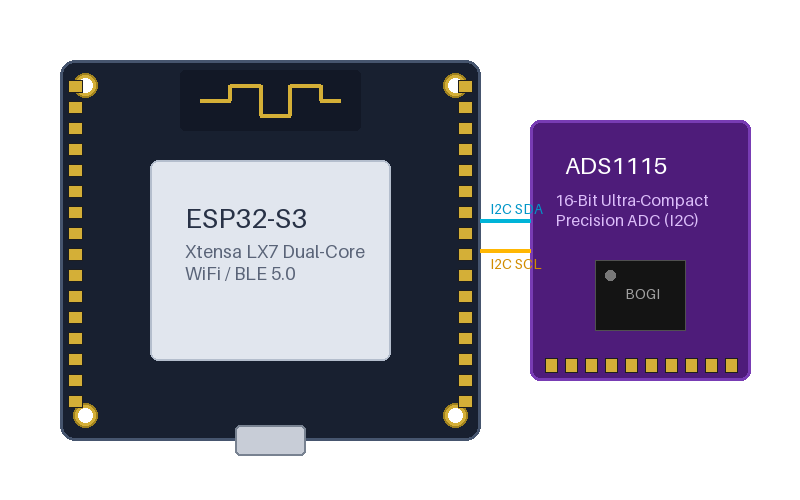
\includegraphics[width=5.0cm, height=2.5cm, keepaspectratio]{assets/controller_ads_board.png}
    };
    \node[align=center] at (2.5, 0) {
      {\bfseries\normalsize Vi điều khiển ESP32-S3 + ADC ADS1115 (16-bit)}\\[3pt]
      {\footnotesize $\bullet$ 2 IC MUX CD74HC4067 quét 21 kênh $\ge$15 Hz}\\[2pt]
      {\footnotesize $\bullet$ Chuỗi lọc số DSP 2 nhánh (Bám nền động \& Ngưỡng 180 mV)}\\[2pt]
      {\footnotesize $\bullet$ Lượng hóa nỗ lực: Bộ ba chỉ số EI -- GAP -- RAL}\\[2pt]
      {\footnotesize $\bullet$ Thuật toán điều khiển trợ lực theo nhu cầu (AAN)}
    };
  \end{tikzpicture}
};

% ==================== TẦNG 3: TẦNG TRỢ LỰC CƠ HỌC ====================
\node[tierCard, fill=t3Bg, below=34pt of t2] (t3) {
  {\bfseries\large\color{amberTitle} TẦNG 3: TẦNG TRỢ LỰC CƠ HỌC (ACTUATION TIER)}\\[6pt]
  \begin{tikzpicture}
    \node[draw=gray!30, fill=white, rounded corners=5pt, inner sep=4pt] (p4) at (-4.5, 0) {
      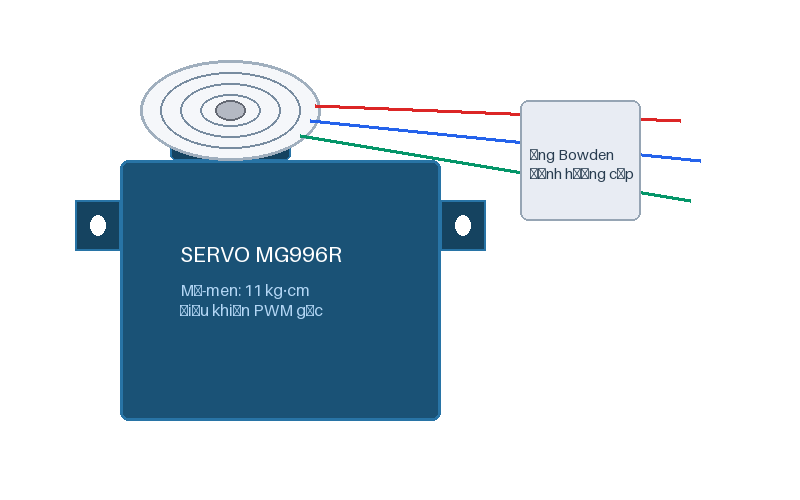
\includegraphics[width=5.0cm, height=2.5cm, keepaspectratio]{assets/servo_spool_assembly.png}
    };
    \node[align=center] at (2.5, 0) {
      {\bfseries\normalsize Cụm 3 Động cơ Servo MG996R \& Tang cuốn cáp}\\[3pt]
      {\footnotesize $\bullet$ Dẫn động cáp Bowden Dyneema kéo gập độc lập 3 ngón}\\[2pt]
      {\footnotesize $\bullet$ Servo chủ động nhả cáp khi chuyển sang chiều duỗi}\\[2pt]
      {\footnotesize $\bullet$ Nẹp đàn hồi hồi vị mu tay hỗ trợ mở khẩu độ tự nhiên}\\[2pt]
      {\footnotesize $\bullet$ Cửa sổ thăm dò tự động phân biệt nỗ lực tự khởi xướng}
    };
  \end{tikzpicture}
};

% ==================== TẦNG 4: TẦNG THỊ GIÁC & TÁC VỤ ====================
\node[tierCard, fill=t4Bg, below=34pt of t3] (t4) {
  {\bfseries\large\color{purpleTitle} TẦNG 4: TẦNG THỊ GIÁC ĐÓN TRƯỚC \& TÁC VỤ (VISION PRE-ACTUATION TIER)}\\[6pt]
  \begin{tikzpicture}
    \node[draw=gray!30, fill=white, rounded corners=5pt, inner sep=4pt] (p5) at (-4.5, 0) {
      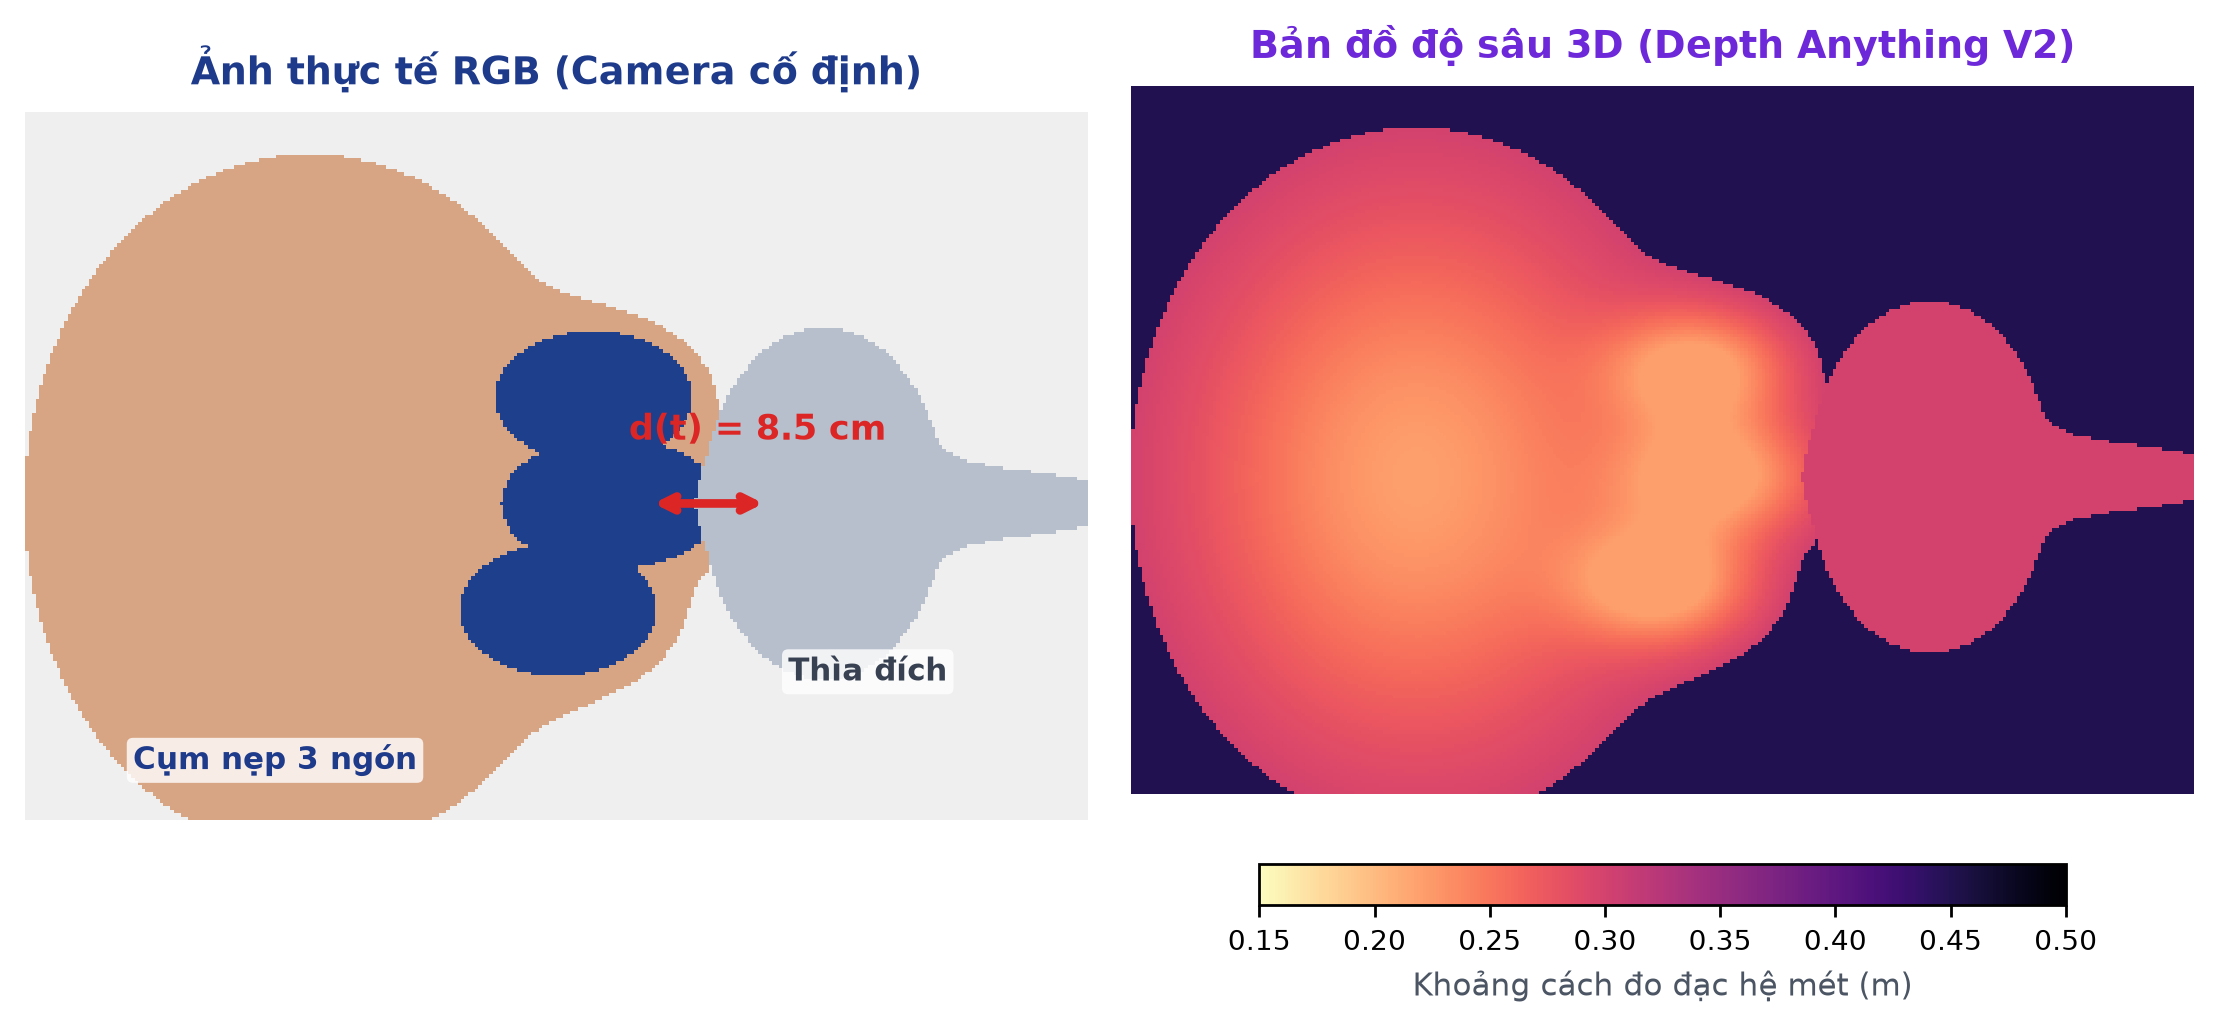
\includegraphics[width=5.2cm, height=2.6cm, keepaspectratio]{assets/depth_anything_scene.png}
    };
    \node[align=center] at (2.5, 0) {
      {\bfseries\normalsize Orange Pi 5 Pro (NPU) + Camera RGB + Depth Anything V2}\\[3pt]
      {\footnotesize $\bullet$ Ước lượng bản đồ độ sâu hệ mét 3D không cần marker}\\[2pt]
      {\footnotesize $\bullet$ Đo cự ly 3D tay -- vật $d(t)$ \& Tính thời gian tới tiếp xúc (TTC)}\\[2pt]
      {\footnotesize $\bullet$ Hỗ trợ định thời chuẩn bị khẩu độ đón trước khi chạm vật}\\[2pt]
      {\footnotesize $\bullet$ Lượng hóa bài tập gắp thìa (Tripod Pinch) \& Phản hồi trực quan}
    };
  \end{tikzpicture}
};

% ==================== MŨI TÊN LIÊN KẾT ĐĂNG ĐỐI ====================
\draw[flowArrow] (t1.south) -- node[tagLbl] {Tín hiệu tương tự 21 kênh (Lực vi sai \& Góc gập)} (t2.north);
\draw[flowArrow] (t2.south) -- node[tagLbl] {Lệnh điều khiển Servo AAN (Kéo gập / Nhả duỗi)} (t3.north);
\draw[biArrow] (t3.south) -- node[tagLbl] {Trạng thái vận động $\longleftrightarrow$ Cự ly 3D \& Định thời TTC đón trước} (t4.north);

\end{tikzpicture}
\end{document}
